\chapter{MÉTODO DE VOLÚMENES FINITOS Y ESQUEMA DE ROE}
A continuación se describen el método y los esquemas a utilizar para llevar a cabo una solución numérica de una ecuación de conservación. La idea principal del capítulo es describir el método de volúmenes finitos y la motivación de su uso. Se explicarán los esquemas adecuados para aplicar el mencionado método, un solucionador del problema de Riemann, denominado esquema de Godunov y otro solucionador aproximado del problema de Riemann, denominado esquema de Roe. Este último es el esquema elegido para resolver las ecuaciones de Euler en este texto.\\
El contenido de este capítulo se basa en el capítulo \textit{Numerical Methods in One Dimension} del texto \cite{LeVequeAstro} y en el capítulo de \textit{Numerical Methods} del texto \cite{LeVeque}, ambos escritos por Randall LeVeque.

\section{Método de volúmenes finitos}
El método de volúmenes finitos (MVF) es un método numérico de integración que se especializa en resolver ecuaciones diferenciales escritas en forma conservativa. El MVF destaca por ofrecer una interpretación peculiar de la función a resolver, ya que es un método basado en la forma \textbf{integral} de las ecuaciones.
\subsection{Discretización del problema}
Al aplicar un método numérico para resolver una ecuación diferencial se necesita discretizar el dominio de la función y la función misma, redefiniendo algunas nociones matemáticas y utilizando aproximaciones. Sea  $D = [a,b]$ el dominio espacial de la solución de una ecuación de conservación. Para aplicar el MVF, este dominio se divide en $N$ intervalos iguales llamados \textbf{celdas}. Cada celda se denomina $\mathcal{C}_i$ y se define como un intervalo, $\mathcal{C}_i = [x_i, x_{i+1}]$. Además, cada celta tiene un ancho $h$ \footnote{La diferencia entre dos puntos sobre el eje $x$ también se denomina $\Delta x$, pero se opta por usar $h$ como símbolo, para evitar escribir ecuaciones engorrosas.}, dado por
\begin{equation}
	h = \frac{b-a}{N}.
\end{equation}
Por lo tanto, se tiene una expresión para el valor de cada $x_i$,
\begin{equation}
	x_i = a + (i-1)h.
\end{equation} 
\begin{figure}[ht]
	\centering
	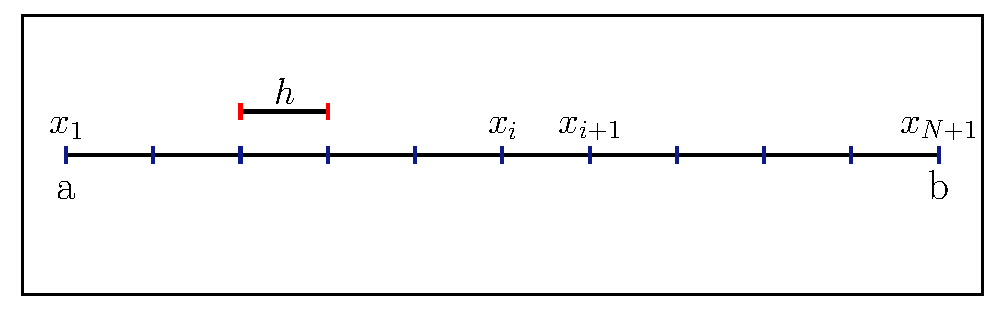
\includegraphics[width=\linewidth]{../some_plots/cap2/graficas/domain.pdf}
	\caption{Esquema de símbolos utilizados para la discretización del dominio espacial. \textbf{Fuente:} elaboración propia.}
	\label{fig:discretizacion-eje-x}
\end{figure}
El dominio temporal, dado por la variable $t$, se discretiza de forma similar. El instante inicial $t_0$ corresponde a $t=0$, de tal manera que cada instante consecuente está separado por un múltiplo entero de una cantidad $k$ denominada \textit{salto temporal}. Por lo tanto, el enésimo instante de tiempo queda como
\begin{equation}
	t_n = nk, \hspace{1cm} \forall n \in \mathbb{N}.
\end{equation}
Para referirse a la función $\mathbf{U}$ discretizada se utilizará una notación especial, esta es,
\begin{equation}
	\mathbf{U}(x_i, t_n) \approx U_{i}^{n}
\end{equation}
que se interpreta como el valor aproximado numéricamente de la función $\mathbf{U}$ en el punto $(x_i, t_n)$. Para conseguir dicha aproximación, el MVF utiliza la siguiente expresión
\begin{equation}
	U_{i}^{n} \approx \frac{1}{h}\int_{x_i}^{x_{i+1}}\mathbf{U}(x, t_n)\dd{x} \equiv \frac{1}{h}\int_{\mathcal{C}_i}\mathbf{U}(x, t_n)\dd{x}
\end{equation}
de tal manera que, aproximadamente, $U_i^n$ toma el valor promedio de $\mathbf{U}(x,t_n)$ \footnote{Para un sistema de conservación, tanto $\mathbf{U}$ como $U$ son vectores. Entonces, formalmente hablando, cada componente de $U$ es aproximadamente el valor promedio de cada componente de $\mathbf{U}$ en una celda $\mathcal{C}_i$.} sobre la celda $\mathcal{C}_i$. Vale la pena destacar que si las funciones $u_j$ de las que depende $\mathbf{U}$ son funciones suaves, la expresión para $U_i^n$ coincide en $\mathcal{O}(h^2)$ con el valor exacto de $\mathbf{U}$ en el punto medio de la i-ésima celda.

\begin{figure}[ht]
	\centering
	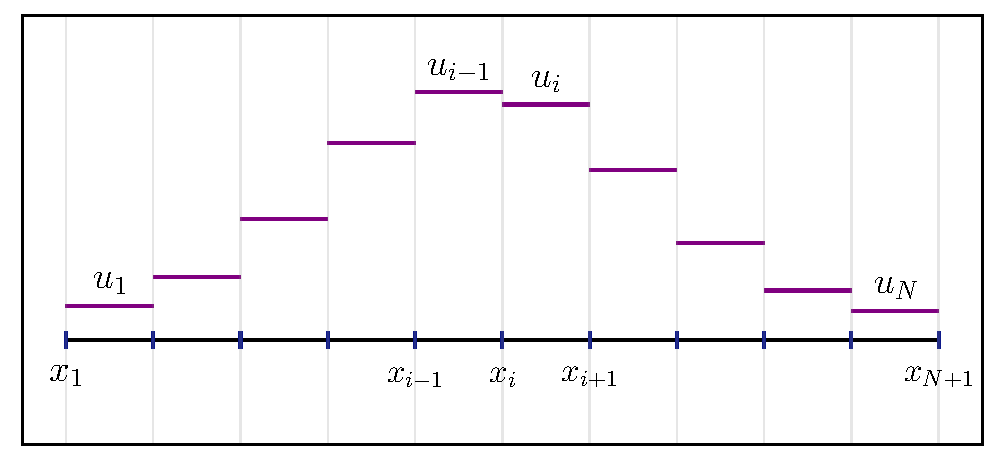
\includegraphics[width=\linewidth]{../some_plots/cap2/graficas/numeric_U.pdf}
	\caption{Gráfica de la construcción de una función escalar numéricamente aproximada $u_i$, en un dominio con pocas celdas. Se puede considerar que una función numéricamente aproximada es una función definida por partes, en donde cada parte es una constante. \textbf{Fuente:} elaboración propia.}
	\label{fig:discretizacion-de-U}
\end{figure}

La ventaja de utilizar un método aproximado basado en los valores promedio de las funciones en las celdas es que éste puede considerarse un método \textbf{conservativo} de tal manera que imite la ley de conservación obtenida a partir de la forma integral de la ecuación de conservación. Esta característica es sumamente importante al considerar ondas de choque como posibles soluciones.

Habiendo considerado la aproximación para obtener $U_i^n$, para continuar con la discretización del problema se puede integrar la ecuación de conservación sobre el dominio $[x_i,x_{i+1}] \times [t_n, t_{n+1}]$, que corresponde a la integral sobre una celda $\mathcal{C}_i$ del dominio espacial y sobre un instante temporal. Utilizando la expresión (\ref{eq:continuidad-2-integral}) se obtiene
\begin{equation}
	\int_{\mathcal{C}_i}\mathbf{U}(x, t_{n+1})\dd{x} - \int_{\mathcal{C}_i}\mathbf{U}(x, t_{n})\dd{x} = \int_{t_n}^{t_{n+1}}\mathbf{F}(\mathbf{U}(x_i,t))\dd{t} - \int_{t_n}^{t_{n+1}}\mathbf{F}(\mathbf{U}(x_{i+1},t))\dd{t}
\end{equation}
\begin{equation}
	\begin{aligned}
		\frac{1}{h}\int_{\mathcal{C}_i}\mathbf{U}(x, t_{n+1})\dd{x} - \frac{1}{h}\int_{\mathcal{C}_i}\mathbf{U}(x, t_{n})\dd{x} = 
		\frac{1}{h}\int_{t_n}^{t_{n+1}}\mathbf{F}(\mathbf{U}(x_i,t))\dd{t} -\\ \frac{1}{h}\int_{t_n}^{t_{n+1}}\mathbf{F}(\mathbf{U}(x_{i+1},t))\dd{t}
	\end{aligned}
\label{eq:integralsobreceldas}
\end{equation}
En esta expresión se puede obtener la diferencia exacta entre dos estados temporales del valor promedio de $\mathbf{U}$. Las integrales del flujo sobre el tiempo no se pueden calcular con exactitud, dado que se necesitaría saber exactamente cómo evoluciona $\mathbf{U}$ con el tiempo. Entonces, se define el flujo aproximado $F_{i-\frac{1}{2}}^n$,
\begin{equation}
	F_{i-\frac{1}{2}}^n \approx \frac{1}{k} \int_{t_n}^{t_n+1} \mathbf{F}(\mathbf{U}(x_i,t)) \dd{t}.
	\label{eq:flujo-numerico}
\end{equation}
Además, se puede usar el hecho de que la información se propaga con velocidad finita a través del espacio, usando las conclusiones del tema del domino de dependencia de una ecuación de conservación. Por lo que se puede asumir que el flujo numérico aproximado $F_{i-\frac{1}{2}}^n$ depende únicamente de los valores de $U$ en las celdas adyacentes,
\begin{equation}
	F_{i-\frac{1}{2}}^n = F(U_{i-1}^n, U_i^n)
\end{equation} 
por esta razón, se utiliza el índice fraccionario para indicar dónde se calcula el flujo $F$. 

\begin{figure}[ht]
	\centering
	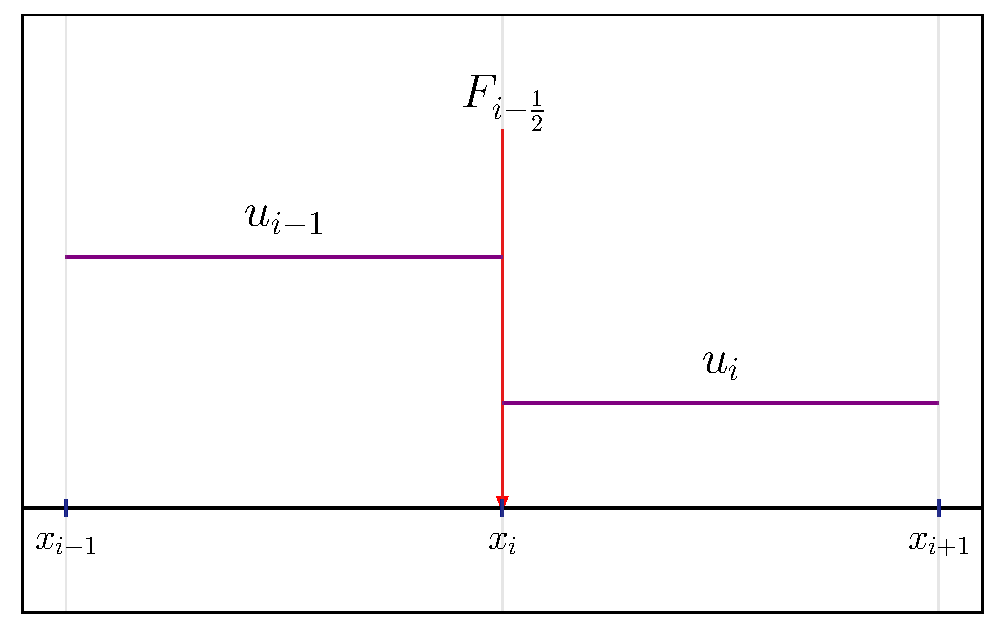
\includegraphics[width=0.9\linewidth]{../some_plots/cap2/graficas/numeric_Flux.pdf}
	\caption{Esquema que muestra que el flujo numérico aproximado $F$ se calcula entre las interfaces de las celdas $\mathcal{C}_i$. \textbf{Fuente:} elaboración propia.}
	\label{fig:flujo-sobre-la-grilla}
\end{figure}

Si es posible promediar adecuadamente el valor del flujo entre las interfaces de las celdas, se podrá construir un método numérico discreto completo. Sustituyendo las expresiones para las aproximaciones numéricas en (\ref{eq:integralsobreceldas}), se obtiene
\begin{equation}
	U_{i}^{n+1}-U_{i}^{n} = 
	\frac{k}{h}\left[ F_{i-\frac{1}{2}} - F_{i+\frac{1}{2}} \right]
	\label{eq:metodo-vol-finitos}
\end{equation}
\begin{equation}
	U_{i}^{n+1}-U_{i}^{n} = 
	\frac{k}{h}\left[ F(U_{i-1}^n, U_i^n) - F(U_{i}^n, U_{i+1}^n) \right]
	\label{eq:metodo-vol-finitos-2}
\end{equation}
de tal manera que se obtiene un método iterativo para calcular $U$ en cualquier instante de tiempo $t_n$.

Como se mencionó previamente, un método numérico de la forma (\ref{eq:metodo-vol-finitos}) es considerado conservativo, dado que imita la propiedad (\ref{eq:integralsobreceldas}) de la solución exacta, pero en forma discreta. Si se suman todos los valores de $U$ y $F$ sobre todas las celdas, desde la celda $\mathcal{C}_L$ hasta la celda $\mathcal{C}_R$ a partir de la expresión (\ref{eq:metodo-vol-finitos-2}), se obtiene
\begin{equation}
 \sum_{i=L}^{R}\left[U_{i}^{n+1}-U_{i}^{n}\right] - 
 \frac{k}{h}\sum_{i=L}^{R}\left[ F(U_{i-1}^n, U_i^n) - F(U_{i}^n, U_{i+1}^n) \right] = 0
\end{equation}
\begin{equation}
	\sum_{i=L}^{R}\left[U_{i}^{n+1}-U_{i}^{n}\right] - 
	\frac{k}{h}\left[F(U_{R-1}^n, U_{R}^n) - F(U_{L}^n, U_{L+1}^n) \right] = 0
\end{equation}
o bien, utilizando la notación de medios enteros
\begin{equation}
	\sum_{i=L}^{R}\left[U_{i}^{n+1}-U_{i}^{n}\right] - \frac{k}{h}\left[F_{R-\frac{1}{2}}^{n} - F_{L+\frac{1}{2}}^{n} \right] = 0.
\end{equation}
A partir de este último resultado se puede concluir que la diferencia entre la suma de los valores de $U$ en un conjunto de celdas consecutivas varía únicamente de acuerdo a los flujos sobre las fronteras de las celdas exteriores. En caso las celdas exteriores fueran las que limitan el dominio completo, se tendrían que invocar las \textbf{condiciones de frontera} adecuadas para el problema a resolver.

\section{Esquemas de flujo numérico}
El método iterativo utilizado para resolver la ecuación de conservación depende de cómo esté definida la función de flujo numérico $F_{i + \frac{1}{2}}^{n}$ en la interfaz entre dos celdas, por lo que es necesario definir un \textbf{esquema} que calcule $F$ basándose en los valores de la función $U$ adyacentes. A continuación se presentan algunos esquemas que proporcionan una función de flujo numérico \textbf{escalar}.

\subsection{Esquema de Lax-Friedrichs}
Para definir una función de flujo numérico aproximada, que dependa de los valores de $u_{i}^{n}$ en dos celdas vecinas, se puede considerar promediar el valor de la función de flujo exacta valuada en los valores de $u$ de ambas celdas, esto es
\begin{equation}
	F(u_{i-1}, u_{i+1}) = \frac{1}{2}\left(f(u_{i-1}) + f(u_{i+	1})\right)
\end{equation}

de tal manera que al sustituir en (\ref{eq:metodo-vol-finitos-2}) se obtiene

\begin{equation}
	u_{i}^{n+1} = u_{i}^{n} 
	+ \frac{k}{2h}\left[ f(u_{i-1}^{n}) - f(u_{i+1}^{n}) \right].
\end{equation}
Sin embargo este esquema no es estable numéricamente para ningún valor de $h/k$. En cambio al usar el siguiente flujo modificado
\begin{equation}
	F(u_{i-1}, u_{i+1}) = \frac{1}{2}\left(f(u_{i-1}) + f(u_{i+	1})\right) + \frac{h}{2k} \left(u_{i-1} - u_{i+1} \right)
	\label{eq:lax-modificado}
\end{equation}
se obtiene el esquema de \textbf{Lax-Friedrichs} al sustituir en (\ref{eq:metodo-vol-finitos-2}), 
\begin{equation}
	u_{i}^{n+1} = \frac{1}{2}\left(u_{i-1}^{n} + u_{i+1}^{n}\right) + \frac{h}{2k} \left(f(u_{i-1}^{n}) - f(u_{i+1}^{n})\right)
\end{equation}

Este esquema produce un flujo correcto a primer orden. El término añadido al flujo en (\ref{eq:lax-modificado}) es un flujo difusivo que funciona agregando una pequeña viscosidad artificial a la dinámica de la solución.\\

A continuación se presentan dos esquemas que se basan en la solución del problema de Riemann en forma exacta y aproximada, respectivamente.

\subsection{Esquema de Godunov}
El esquema propuesto por Godunov consiste básicamente en resolver el problema de Riemann de la ecuación de conservación en cuestión para cada celda del dominio con el objetivo de calcular el flujo numérico adecuado en las interfaces de las celdas. La ventaja de este esquema es que al resolver el problema de Riemann en distintos intervalos espaciales, este método resulta ser conservativo, puesto que la solución al problema de Riemann satisface la ecuación de conservación como una solución débil.

El esquema de Godunov define una función por partes $\tilde{u}^{n}(x,t_n)$ que toma el valor de $u_{i}^{n}$ para cada $x \in \mathcal{C}_i$ como un valor constante (La idea de interpretar a $u_{i}^{n}$ como una función por partes fue discutida en la figura (\ref{fig:discretizacion-de-U})), y está definida para un intervalo temporal $t_{n}\leq t \leq t_{n+1}$. De tal manera que $\tilde{u}^{n}(x,t_n)$ se toma como la condición inicial para resolver la ecuación de conservación en cuestión en dicho intervalo de tiempo, por tanto, resolviendo una secuencia de problemas de Riemann.

Ya que la idea de un esquema numérico el contexto de los métodos de volúmenes finitos es producir un flujo numérico adecuado, el esquema de Godunov redefine la función de flujo aproximado (\ref{eq:flujo-numerico}) como la integral del flujo exacto en la coordenada $x_i$ dado al valuar la  la función por partes $\tilde{u}^{n}(x,t_n)$ en la función de flujo, esto es
\begin{equation}
	F_{i-\frac{1}{2}}^{n} = \frac{1}{k}\int_{t_n}^{t_{n+1}}f(\tilde{u}^{n}(x_i,t))\dd{t}.
\end{equation}
La diferencia entre esta integral y la definida en (\ref{eq:flujo-numerico}) es que la última es trivial de resolver. Esto se justifica con el hecho de que todas las soluciones al problema de Riemann en $x=x_{i}$ son soluciones de \textbf{similitud}, i.e., son constantes en las rectas dadas por $(x-x_{i})/t = c$, con $c$ constante. Entonces, $\tilde{u}^{n}(x_{i},t)$ es constante en el tiempo y la integral es trivial.

Sea $u^{*}(u_L; u_R)$ la solución al problema de Riemann sobre la recta $x/t = 0$, que se obtiene con la siguiente condición inicial
\begin{equation}
	u(x,0) = 
	\begin{cases}
		u_L & \text{si } x < 0 \\
		u_R & \text{si } x > 0
	\end{cases}
\end{equation}
entonces, se define a $\tilde{u}^{n}(x,t)$ como
\begin{equation}
	\tilde{u}^{n}(x_{i},t) \equiv u^{*}(u_{i-1}^{n} ; u_{i}^{n}).
\end{equation}
Entonces, el flujo numérico se reduce a
\begin{equation}
	F(u_{i-1}^{n}, u_{i}^{n}) = f(u^{*}(u_{i-1}^{n} ; u_{i}^{n}))
\end{equation}
y el esquema de Godunov aplicado al MVF resulta en
\begin{equation}
	u_{i}^{n+1} = u_{i}^{n} + \frac{h}{k} \left[f(u^{*}(u_{i-1}^{n} ; u_{i}^{n})) - f(u^{*}(u_{i}^{n} ; u_{i+1}^{n}))\right].
\end{equation}

\subsubsection{Esquema de Godunov para el caso escalar}
Para definir la función $u^{*}(u_L; u_R)$ basta con recordar que el problema de Riemann tiene una solución que corresponde a una discontinuidad que se traslada con una velocidad $s=\frac{f(u_L)-f(u_R)}{u_L - u_R}$, de acuerdo a la condición Rankine - Hugoniot. Por tanto, es conveniente proponer una solución de este tipo para $u^{*}$; 
\begin{equation}
	u^{*}(u_L; u_R) = 
	\begin{cases}
		u_L & \text{si } s \geq 0\\
		u_R & \text{si } s < 0.
	\end{cases}
\end{equation}
Sin embargo, esta construcción no garantiza que se satisface la condición de entropía.	

\subsubsection{Condición de estabilidad del esquema de Godunov}
Ahora bien, es posible que el valor de la solución $\tilde{u}^{n}(x_{i},t)$ no sea constante en $x_i$ por el efecto de otras ondas que se propagan e interferirían con la solución. Sin embargo, las velocidades de las ondas están limitadas a los autovalores de la matriz jacobiana $f'(u)$ y dado que los intervalos que separan cada dominio en que se resuelve cada problema de Riemann independiente están separados por una distancia $h$, se puede asumir que $\tilde{u}^{n}(x_{i},t)$ será constante en el intervalo de tiempo $[t_n, t_{n+1}]$ siempre que $k$ sea lo suficientemente pequeño. Matemáticamente, esto se describe como
\begin{equation}
	\left|\frac{h}{k} \lambda_{p}(u_i^{n})\right| \leq 0
\end{equation}
para todos los autovalores $\lambda_{p}$ en cada $u_i^{n}$. En el caso escalar, esta condición se reduce a
\begin{equation}
	\left|\frac{h}{k} f'(u_i^{n})\right| \leq 0.
\end{equation}
